%%-------------------------------------------------------------------------------------- Início
\section{Teste do Ambiente de Trabalho}
\begin{frame}[allowframebreaks,fragile,t]{Teste do Ambiente de Desenvolvimento}
  \begin{enumerate}
    \item Crie a aplicação \verb!Rails! \alert{agenda}.
    \begin{lstlisting}[style=BashInputStyle]
	  $ mkdir Workspace
	  $ cd Workspace
	  $ rails new agenda
    \end{lstlisting}
 
    \item Crie o banco de dados \alert{agenda}, ainda sem nenhuma tabela.
    \begin{lstlisting}[style=BashInputStyle]
	  $ cd agenda
	  $ rake db:create
    \end{lstlisting}

    \item Inicie o servidor web de desenvolvimento que acompanha o Rails.
    \begin{lstlisting}[style=BashInputStyle]
	  $ rails server
    \end{lstlisting}

\framebreak
    \item Digite o endereço \alert{\url{http://localhost:3000}} no navegador web, uma página 
      de boas-vindas da aplicação deverá ser apresentada.
    \begin{figure}[h!]
	\centering
	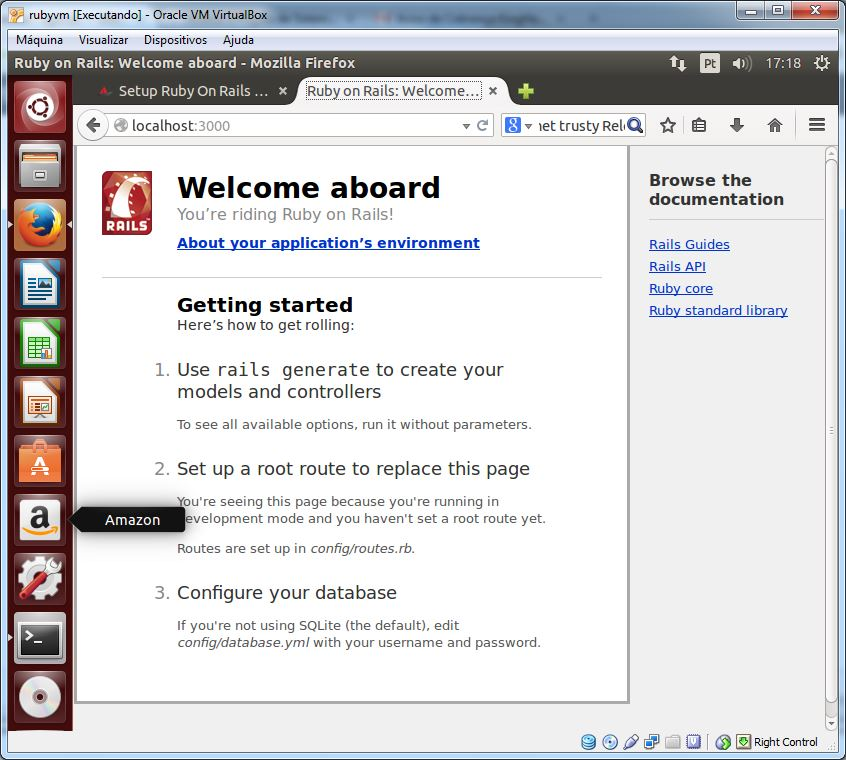
\includegraphics[width=0.45\textwidth]{devops/imagens/rails-boas-vindas.jpg}
    \end{figure}

\framebreak
    \item Inicialize o repositório git local.
    \begin{lstlisting}[style=BashInputStyle]
	  $ cd ~/Workspace/agenda
	  $ git init
    \end{lstlisting}
 
    \item Inclua todos os arquivos da aplicação no repositório local e efetive 
      a gravação deles.
    \begin{lstlisting}[style=BashInputStyle]
	  $ git add .
	  $ git commit -m "Initial commit."
    \end{lstlisting}

    \item Vincule o repositório local ao repositório remoto no Bitbucket.org.
    \begin{lstlisting}[style=BashInputStyle]
	  $ git remote add origin EnderecoDoSeuRepositorio
    \end{lstlisting}
    
    \item Envie os arquivos do repositório local para repositório remoto no Bitbucket.org utilizando
      o comando a seguir e, após isso, visualize-os no \verb!Dashboard! do \url{http://bitbucket.org}.
    \begin{lstlisting}[style=BashInputStyle]
	  $ git push -u origin master
    \end{lstlisting}
     
  \end{enumerate}
\end{frame}
